\chapter{Conclusão}
\label{Conclusao}


Foi desenvolvida uma primeira versão funcional (1.0) do sistema \textit{Web} \textit{e-Plano} para facilitar o preenchimento do Plano Semestral de Trabalho Docente, o qual é um instrumento de planejamento ao mesmo tempo para o docente e para a gestão do \acf{DAA} do \ac{IFG}.

Sendo um documento oficial auditável, é imperativo que o Plano Semestral de Trabalho Docente esteja coerente com a norma.
A aplicação garante ao docente e ao gestor, por meio da aplicação das \nameref{RegrasDeNegocio}, a conformidade do Plano Semestral de Trabalho Docente com a Resolução nº 9 do \ac{IFG}.

Utilizando tecnologias atuais do mercado de trabalho foi possível aplicar neste Trabalho de Conclusão de Curso uma variedade de conhecimentos adquirido ao longo do curso de Tecnologia em Análise e Desenvolvimento de Sistemas de forma integrada.
A experiência do desenvolvimento em uma situação de demanda real com prazos e recursos definidos foi fundamental para uma formação integral.

Melhorias planejadas da aplicação, incluem uma funcionalidade de envio de \textit{e-mail} para que o usuário receba o link de acesso ao formulário salvo, que pode ser visto na figura \ref{fig:prot10} de protótipo.
Além disso, é intenção o uso de um \textit{login} utilizando o serviço de autenticação do IFG via \textit{Web Service}, o qual depende da liberação por parte da Diretoria de Tecnologia da Informação.
Uma alternativa local para implantação está sendo construída usando o deploy via ``Docker container''~\footnote{http://dockerhub.com}.

\begin{figure}[htb]
    \centering
    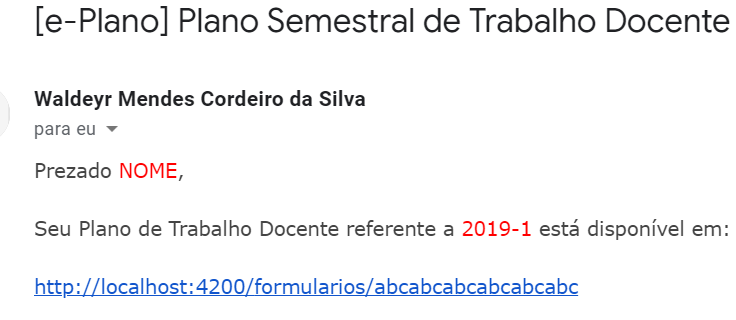
\includegraphics[width=0.5\textwidth]{img/email.PNG}
    \caption[Protótipo 10: \textit{E-mail}]{Protótipo 10: \textit{E-mail enviado pelo sistema para acesso ao Plano Semestral de Trabalho Docente}.}
    \label{fig:prot10}
\end{figure}